%!TEX root = ../../../super_main.tex
\subsection{Consistent Dialogs}
\label{sec:consistent_dialogs}

The pop-up dialogs have undergone a major overhaul during the second sprint. The previously implemented dialog (\androidinline{GDialog} see \figref{fig:gdialog}) was found to be inconsistent with the \giraf design manual. The overall idea was that all dialogs, across the \giraf-software suite, should be replaced with standard dialogs in order the give a consistent experience. 

\begin{figure}[!htbp]
    \centering
    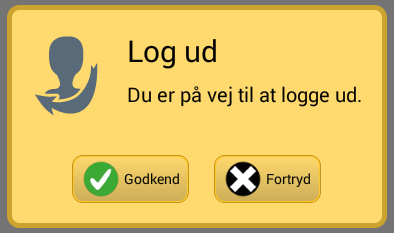
\includegraphics[width=0.4\textwidth]{sprint_two/giraf_components/gdialog}
    \caption{Old confirm dialog}
    \label{fig:gdialog}
\end{figure}

\subsubsection{Design}
We found that there was need for multiple common types of dialogs. The first being a simple notification dialog, which includes a title, a message, and a button for closing the dialog. The second is a confirmation dialog as seen in \figref{fig:giraf_confirm_dialog} that provides an extra confirmation button and the possibility to provide an action for that button. In general it should be possible to add many buttons to a dialog for other use cases. It should also be possible to have a dialog that can have more customizable content then just buttons and text. All of these dialogs should be able to close by clicking outside the dialog.

\begin{figure}[!htbp]
    \centering
    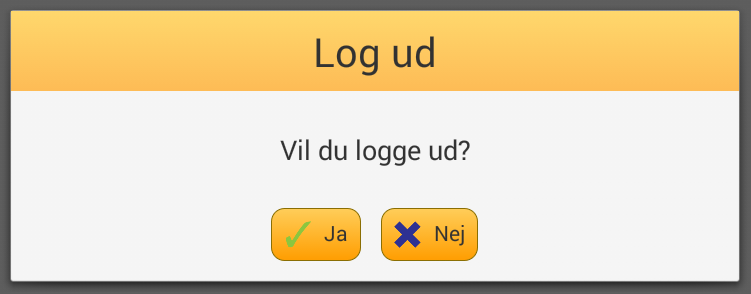
\includegraphics[width=0.7\textwidth]{sprint_two/giraf_components/giraf_confirm_dialog}
    \caption{Redesigned confirm dialog}
    \label{fig:giraf_confirm_dialog}
\end{figure}

\subsubsection{Implementation}

All dialogs should ideally look similar to provide a consistent experience. This was achieved by letting all dialogs inherit from the same abstract class called \androidinline{GirafDialog} which implements functionality and visuals used in all the subclasses. Some specialized classes of the dialog, for the various use cases, were implemented for convenience. The general approach for callback from these classes is that the developer should implement a callback interface on the calling \androidinline{Activity} which the dialog will keep a reference to.